\begin{figure}
\centering

\def\picScale{0.08}    % define variable for scaling all pictures evenly
\def\colWidth{0.5\linewidth}

{\includegraphics[width=0.95\linewidth]{figures/FREEhand.jpg}} %\fill[blue] (0,0) circle (2pt);

\begin{tikzpicture} %[every node/.style={draw=black}]
% \draw[help lines] (0,0) grid (4,2);
\matrix [row sep=0cm, column sep=0cm, style={align=center}] (my matrix) at (0,0) %(2,1)
{
\node[style={anchor=center}] {\includegraphics[width=\colWidth]{figures/photos/labFREEs3.jpg}}; %\fill[blue] (0,0) circle (2pt)
&
\node[style={anchor=center}] {\includegraphics[width=\colWidth, height=160pt]{figures/stewartRender.png}}; %\fill[blue] (0,0) circle (2pt);
\\
};

%\node[style={anchor=center}] at (0,-5) (FREEstate) {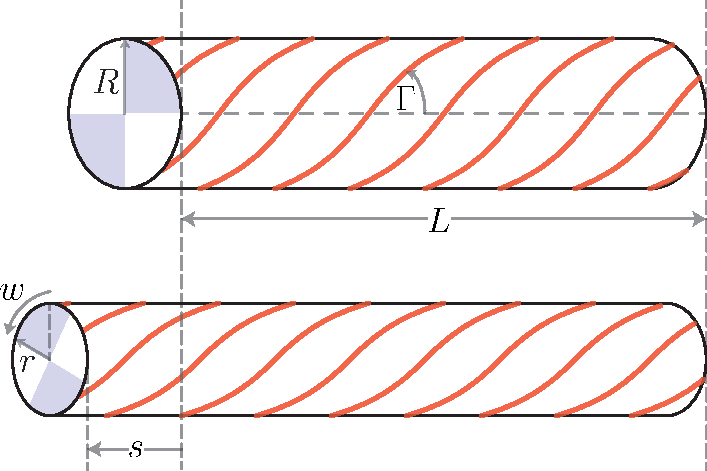
\includegraphics[width=0.7\linewidth]{figures/FREEstate_noLabels2.pdf}};

\end{tikzpicture}

\caption{A fiber-reinforced elastomeric enclosure (FREE) (top) is a soft fluid-driven actuator composed of an elastomer tube with fibers wound around it to impose deformation in specific directions upon pressurization, such as extension and torsion. In this paper we explore the potential of combining multiple FREEs in parallel to achieve fully controllable multi-dimensional soft actuation, such as in a parallel arrangement around a flexible spine element (bottom-left), or a Stewart Platform arrangement (bottom-right).}
\label{fig:overview}
\end{figure}




% DELETED IMAGE%%%%%%%%%%%%%%%%%%%%%%%%%%%%%%%%%%%%%%%%%%%%%%%%%%%
%
%\node[style={anchor=center}] {\includegraphics[width=\colWidth]{figures/FREEhand.png}}; %\fill[blue] (0,0) circle (2pt);
%&
%\node[style={anchor=center}] {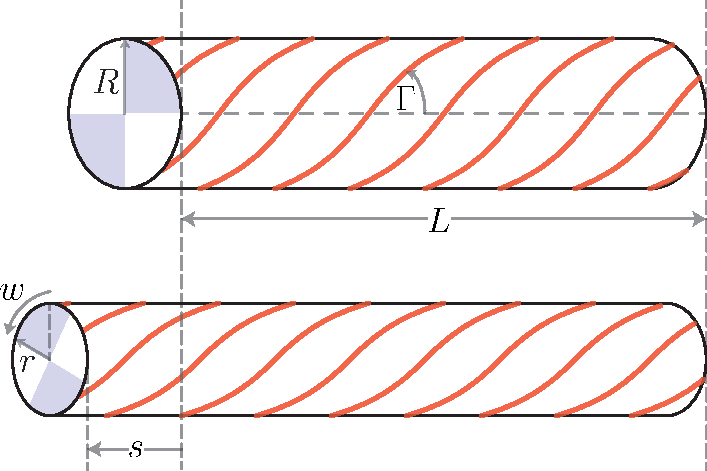
\includegraphics[width=\colWidth]{figures/FREEstate_noLabels2.pdf}}; %\fill[blue] (0,0) circle (2pt);
%
%\\
% A pressurized fiber reinforced elastomeric enclosure (FREE);